\documentclass[12pt,oneside]{krantz}
\usepackage{lmodern}
\usepackage{amssymb,amsmath}
\usepackage{ifxetex,ifluatex}
\usepackage{fixltx2e} % provides \textsubscript
\ifnum 0\ifxetex 1\fi\ifluatex 1\fi=0 % if pdftex
  \usepackage[T1]{fontenc}
  \usepackage[utf8]{inputenc}
\else % if luatex or xelatex
  \ifxetex
    \usepackage{mathspec}
  \else
    \usepackage{fontspec}
  \fi
  \defaultfontfeatures{Ligatures=TeX,Scale=MatchLowercase}
\fi
% use upquote if available, for straight quotes in verbatim environments
\IfFileExists{upquote.sty}{\usepackage{upquote}}{}
% use microtype if available
\IfFileExists{microtype.sty}{%
\usepackage[]{microtype}
\UseMicrotypeSet[protrusion]{basicmath} % disable protrusion for tt fonts
}{}
\PassOptionsToPackage{hyphens}{url} % url is loaded by hyperref
\usepackage[unicode=true]{hyperref}
\hypersetup{
            pdftitle={Herobrine Returns},
            pdfauthor={Beckett Stephens},
            pdfborder={0 0 0},
            breaklinks=true}
\urlstyle{same}  % don't use monospace font for urls
\usepackage{natbib}
\bibliographystyle{plainnat}
\usepackage{longtable,booktabs}
% Fix footnotes in tables (requires footnote package)
\IfFileExists{footnote.sty}{\usepackage{footnote}\makesavenoteenv{long table}}{}
\usepackage{graphicx,grffile}
\makeatletter
\def\maxwidth{\ifdim\Gin@nat@width>\linewidth\linewidth\else\Gin@nat@width\fi}
\def\maxheight{\ifdim\Gin@nat@height>\textheight\textheight\else\Gin@nat@height\fi}
\makeatother
% Scale images if necessary, so that they will not overflow the page
% margins by default, and it is still possible to overwrite the defaults
% using explicit options in \includegraphics[width, height, ...]{}
\setkeys{Gin}{width=\maxwidth,height=\maxheight,keepaspectratio}
\IfFileExists{parskip.sty}{%
\usepackage{parskip}
}{% else
\setlength{\parindent}{0pt}
\setlength{\parskip}{6pt plus 2pt minus 1pt}
}
\setlength{\emergencystretch}{3em}  % prevent overfull lines
\providecommand{\tightlist}{%
  \setlength{\itemsep}{0pt}\setlength{\parskip}{0pt}}
\setcounter{secnumdepth}{5}
% Redefines (sub)paragraphs to behave more like sections
\ifx\paragraph\undefined\else
\let\oldparagraph\paragraph
\renewcommand{\paragraph}[1]{\oldparagraph{#1}\mbox{}}
\fi
\ifx\subparagraph\undefined\else
\let\oldsubparagraph\subparagraph
\renewcommand{\subparagraph}[1]{\oldsubparagraph{#1}\mbox{}}
\fi

% set default figure placement to htbp
\makeatletter
\def\fps@figure{htbp}
\makeatother

\usepackage{booktabs}
\usepackage{caption}
\captionsetup[figure]{labelformat=empty}

\title{Herobrine Returns}
\providecommand{\subtitle}[1]{}
\subtitle{Book 4}
\author{Beckett Stephens}
\date{2018-06-04}

\begin{document}
\maketitle

{
\setcounter{tocdepth}{1}
\tableofcontents
}
\chapter*{Preface}\label{preface}


\begin{figure}
\centering
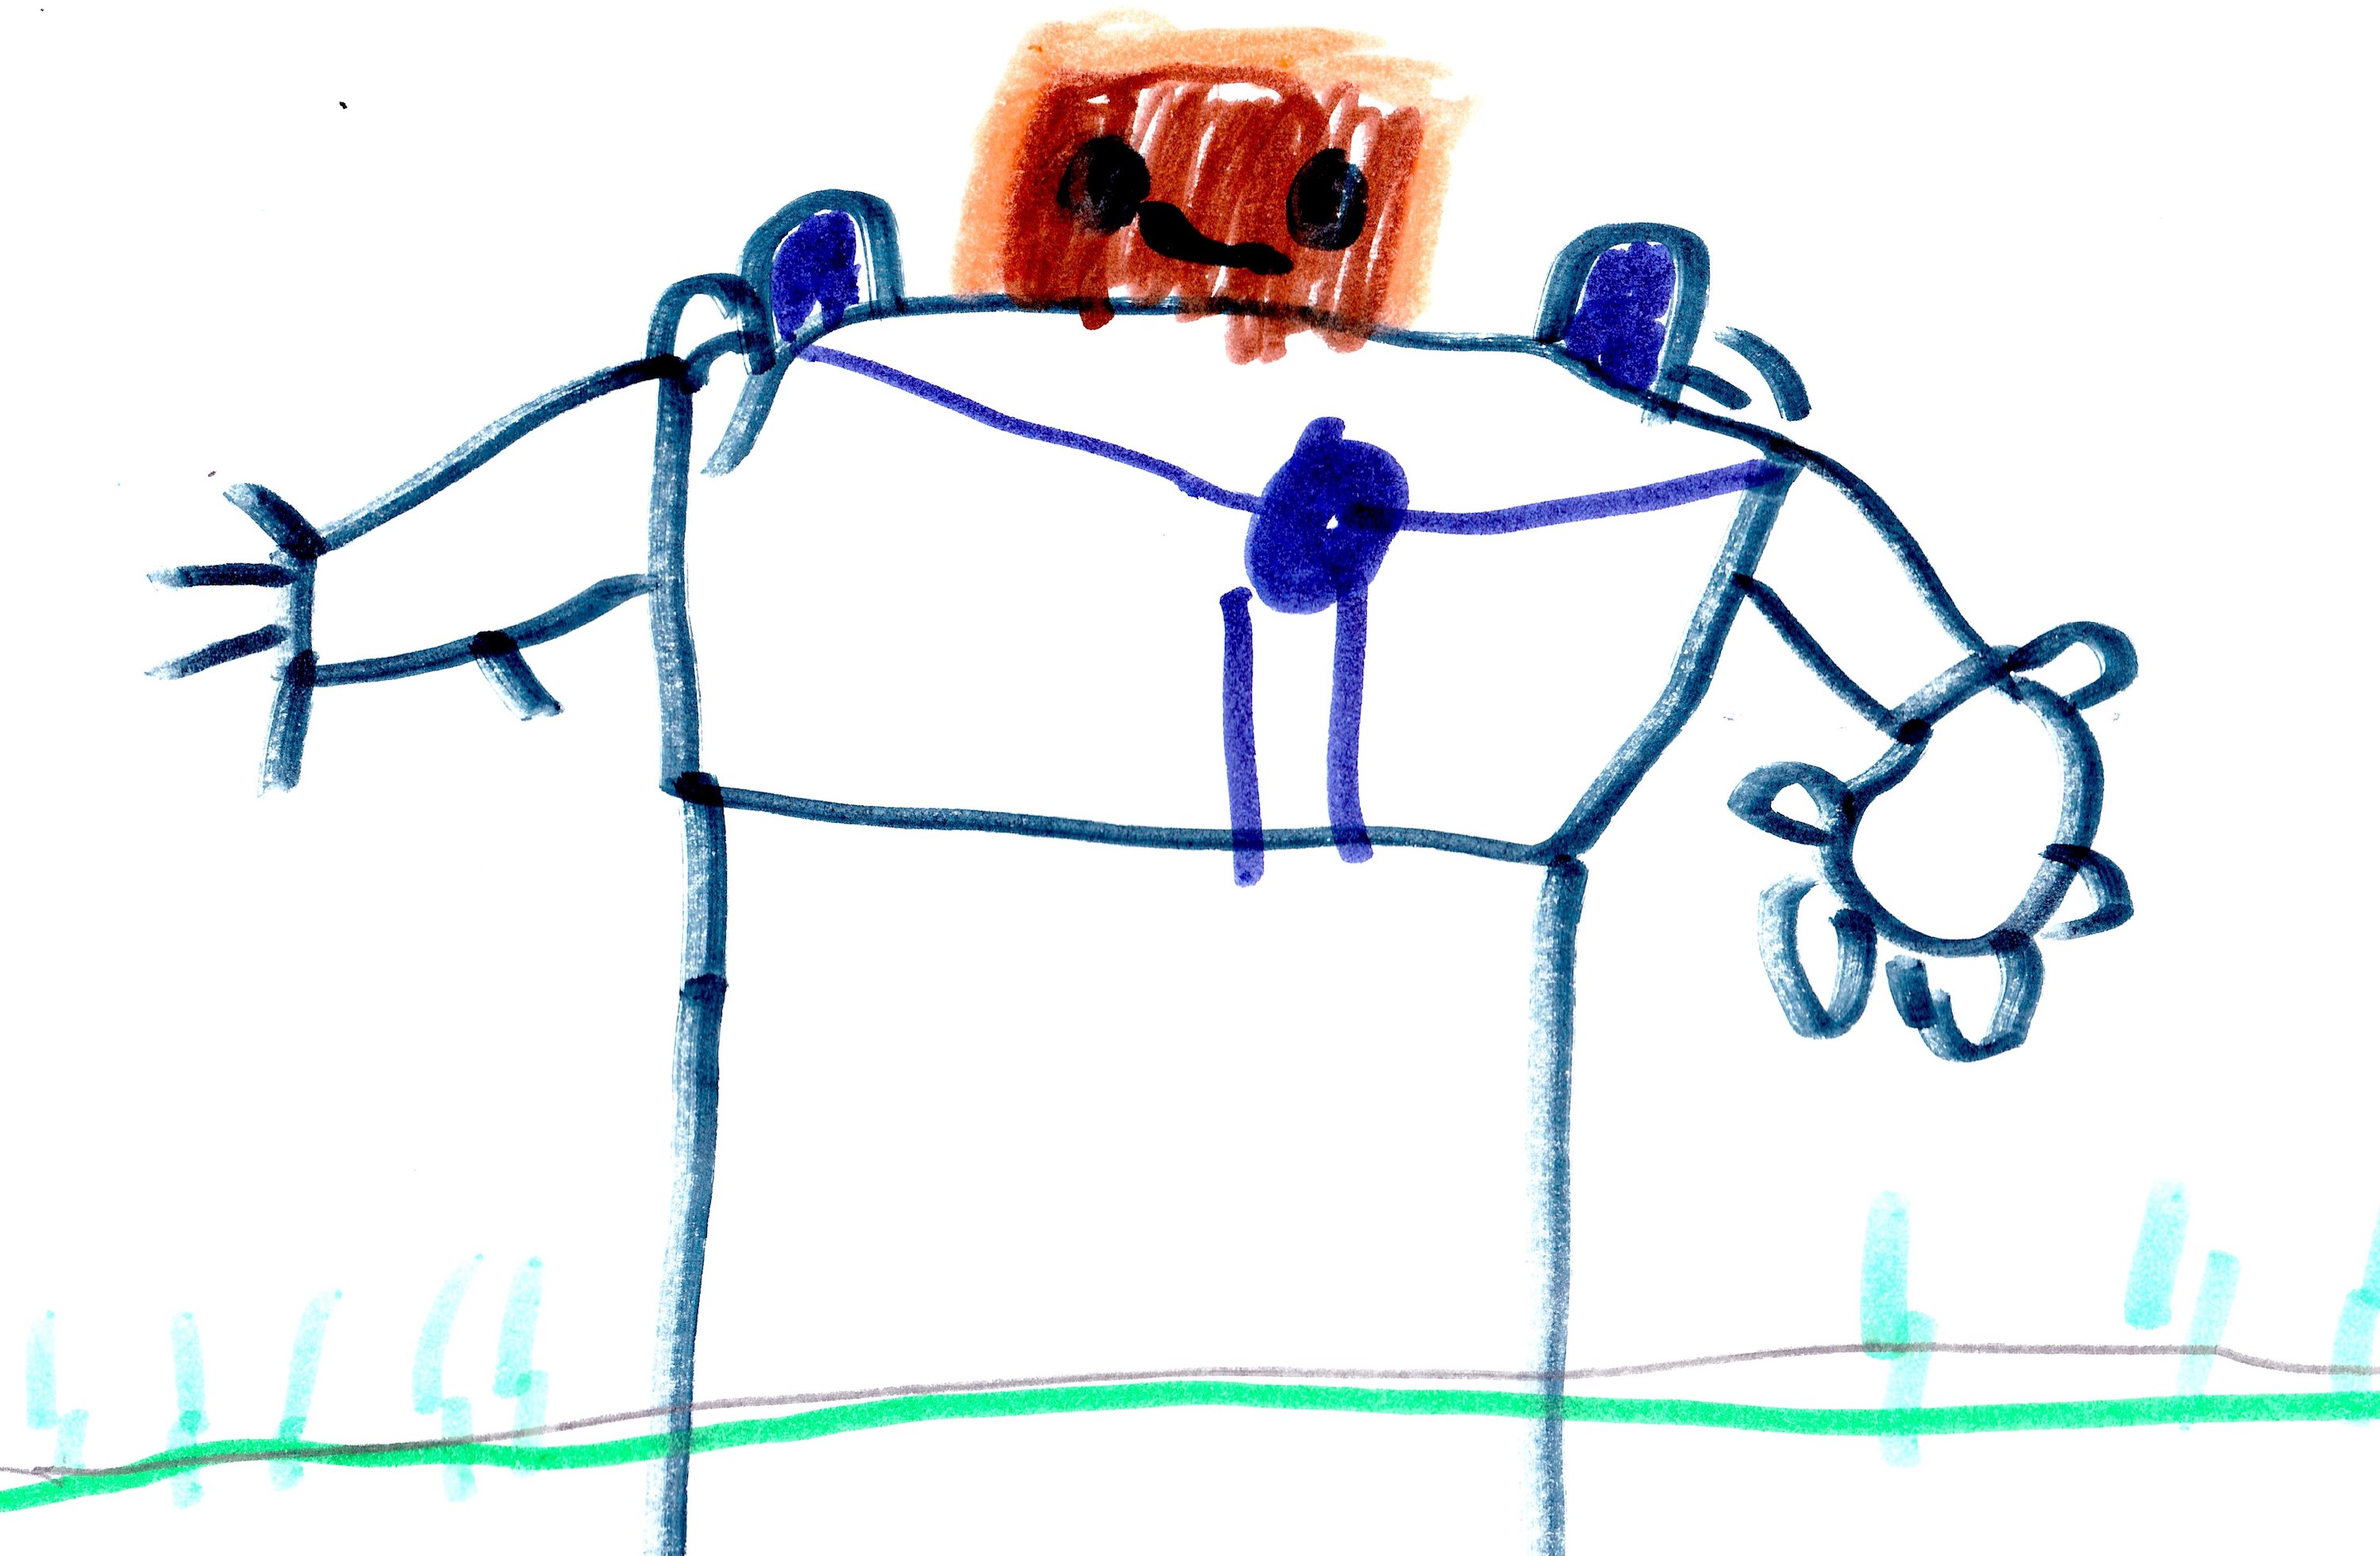
\includegraphics{img/1-herobrine-medium.jpg}
\caption{}
\end{figure}

This book is about my adventures in a video game named Minecraft.

\chapter*{About the Author}\label{about-the-author}


Beckett Stephens is an aspiring author and illustrator. \emph{Herobrine
Returns} is his third published work. Beckett also loves Minecraft,
Lego's, and Transformers, as well as making up endless stories while he
walks. He currently lives in Maryland with his younger brother.

\chapter*{Acknowledgements}\label{acknowledgements}


Thanks to Dad for helping me publish \emph{Herobrine Returns} online.
Also, thanks to Minecraft community for the inspiration that helped me
make this book.

\chapter{Herobrine Returns}\label{herobrine-returns}

\begin{figure}
\centering
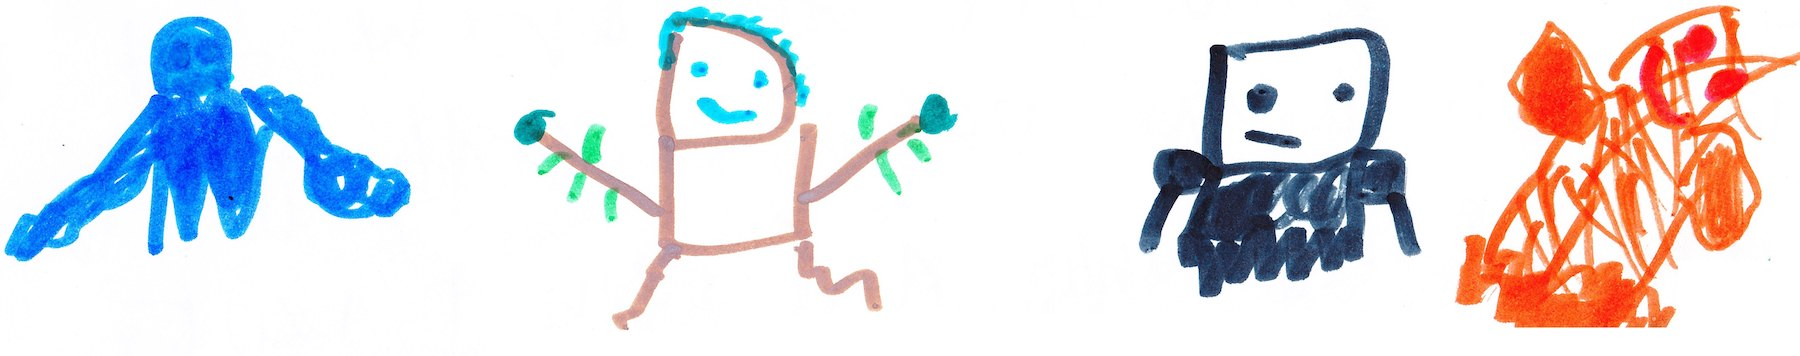
\includegraphics[width=6.25000in]{img/3-gods.jpg}
\caption{}
\end{figure}

Herobrine came out and said, ``Come and get me!'' I said, ''No.''
Herobrine said, ``I just wanted you to get a look at me. I will come
back in an hour to kill you.'' Then he went away.

\emph{At my base\ldots{}}

I said, ``Malek, what data did you collect?'' Malek said, ``The gems we
have can turn us into gods. The bad guys want to get the gems so they
can turn into gods.''

\emph{One hour later\ldots{}}

Herobrine came out of the portal. My team and I got out of my base. The
fight was long but at the end I turned into the Life God. That guy's
weakness is things that contain good magic like trees, good guys and
basically earth. I almost shut off Herobrine but he ran away before I
could deactivate him. After that I took a nap. When I woke up I said,
``It's time we raid Herobrine's base.''

\chapter{We Raid the Base}\label{we-raid-the-base}

Everybody was silent then Malek said, ``Are you crazy? That's
impossible! People come in and then die.'' I said, ``My grandfather
found out and in every End Temple there's a tunnel that leads right to
Herobrine's base.''

\emph{In the tunnel\ldots{}}

I said, ``Our job is to blow up Herobrine's base. While we are inside
getting all the information, King Creeper, Alex, and Aden will construct
a bomb. When the bomb is finished you come inside and blow up
Herobrine's base.''

\emph{On Earth\ldots{}}

Steve Decided to go to the end to see Alex, his wife.

\emph{In the End\ldots{}}

Malek, Felix, and I got in Herobrine's base. Felix and I got in the
vent, and Malek pretended to be a bad guy. I saw Cindy come out of a
door and took a picture of her membership card.

\begin{figure}
\centering
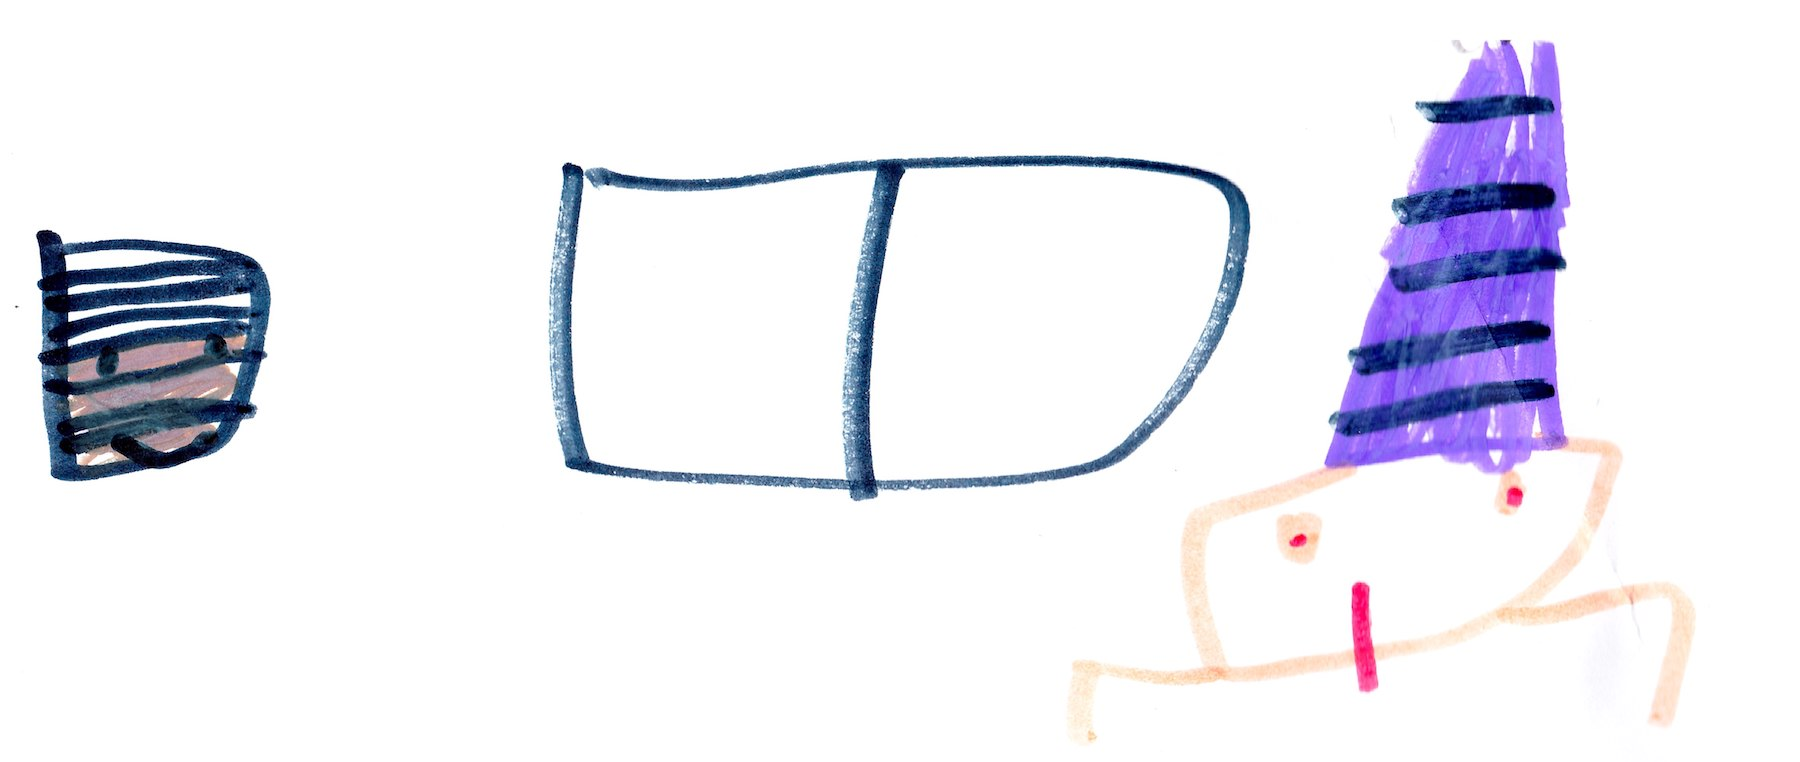
\includegraphics[width=6.25000in]{img/7-door.jpg}
\caption{}
\end{figure}

\emph{In the bad guy's base\ldots{}}

Felix was in a fight with Will. When the fight ended, Felix was put in
prison.

\emph{In the tunnel\ldots{}}

Aden, King Creeper, and Alex were almost done, but a sinkhole opened,
and Aiden and the bomb fell Down. Aden died.

\emph{In the bad guy's base\ldots{}}

Malek accidentally found Will who said, ``Malek? Is it really you?
Guards, get him!'' Malek said, ``I knew this was a bad idea''. Malek was
put in prison.

\emph{In the tunnel\ldots{}}

Sinkholes were everywhere. Alex saw Steve, and Steve made a portal. Alex
and Steve went back to Earth. Eventually King creeper made it to
Herobrine's base. He freed Malek and Felix. King creeper called me and
said, ``Time to blow up the base!'' I said, ''But there's no bomb you
will have to blow yourself up.'' King Creeper said, ``Then that's what
I'll do,'' and everyone got out. King Creeper exploded but did not come
back to life. I started to cry. I felt like my team was falling apart,
but also I had to stay sharp.

\chapter{The Bad Guy Survival on
Earth}\label{the-bad-guy-survival-on-earth}

\begin{figure}
\centering
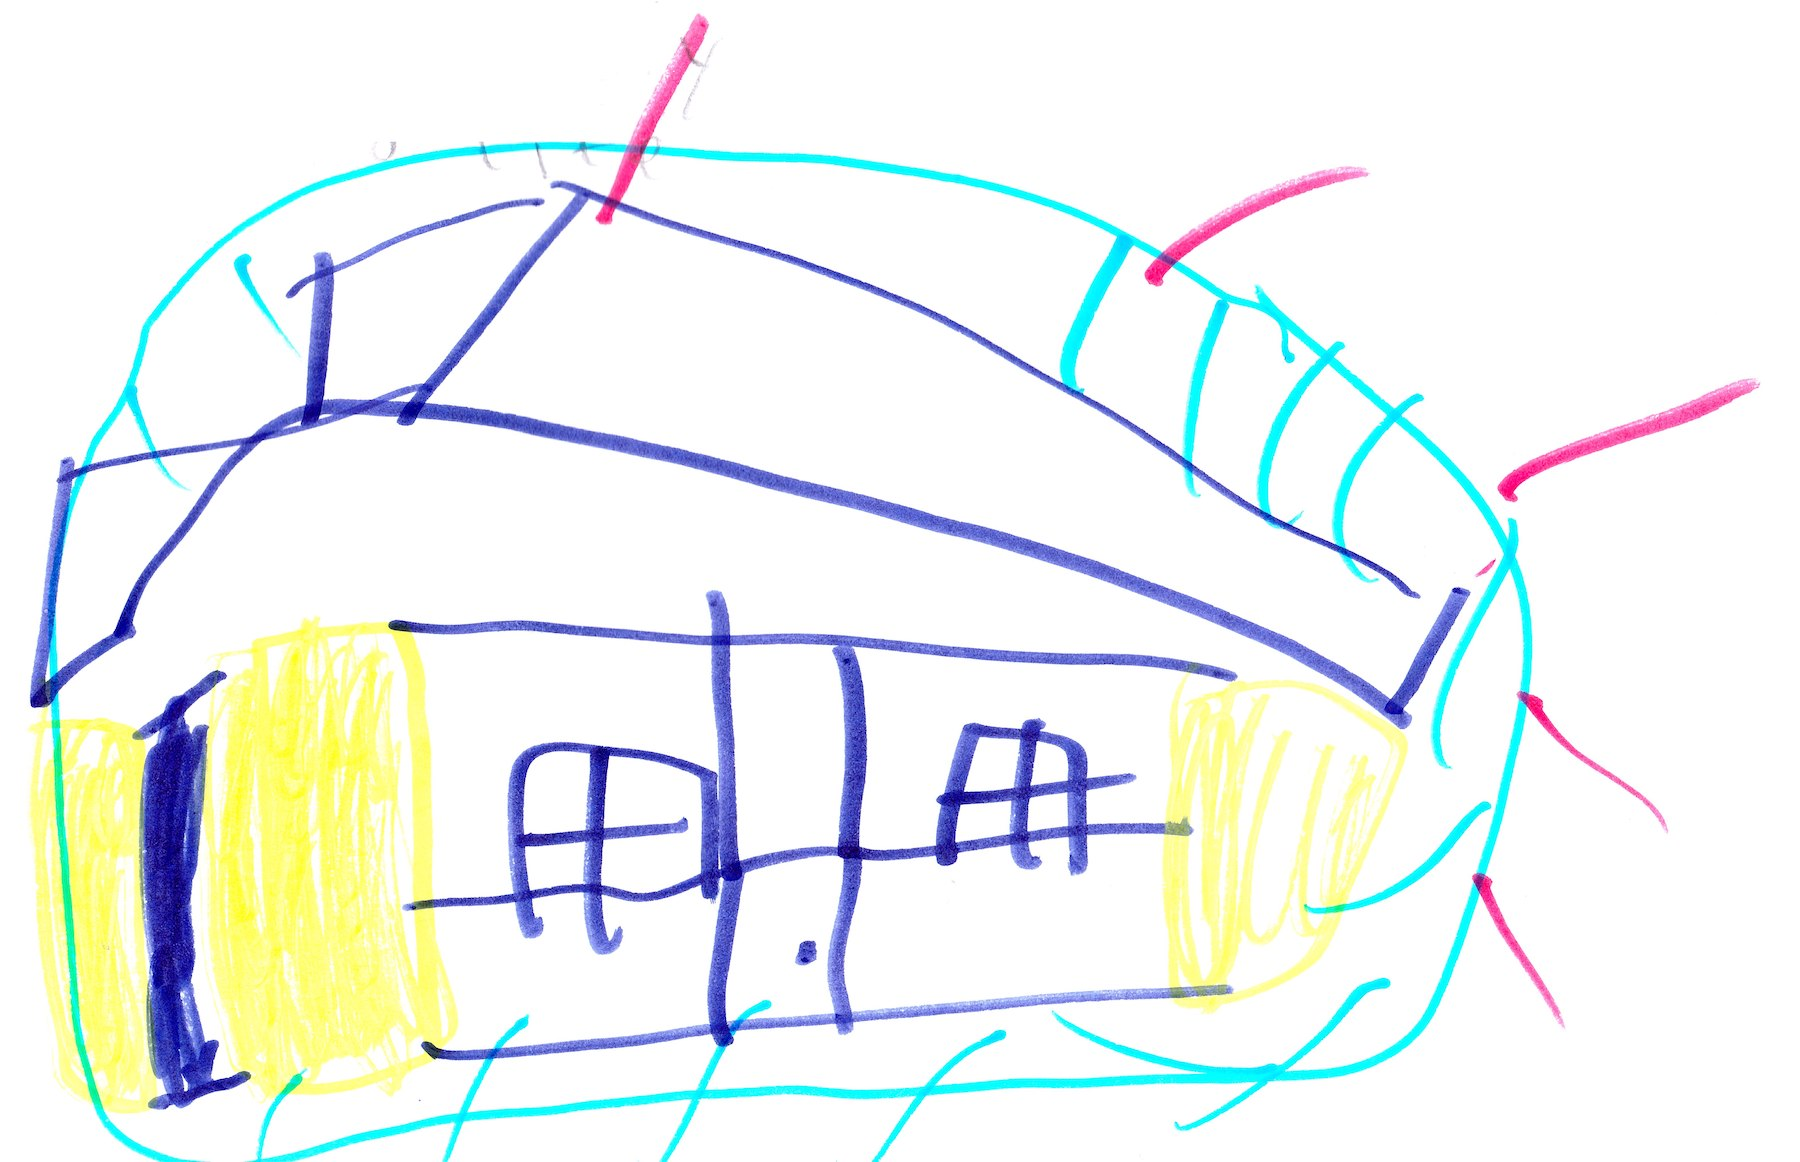
\includegraphics[width=6.25000in]{img/10-base.jpg}
\caption{}
\end{figure}

It would take a year to fix the base in the End. After the base was
destroyed, Herobrine put his base on Earth. Since Herobrine has never
lived on earth it was hard to survive. Herobrine was always mad on
Earth.

One day Cindy was sent to the mines. Cindy found our Mineshaft and went
inside. She found a door and opened it. Inside was where we found King
Creeper but this time it was all decorated with zombie decorations.
Cindy looked around and then she heard someone say in a deep voice,
``Cindy, I was looking for you.'' Cindy said, ``King Zombie!''

\chapter{The Battle of Our Lives}\label{the-battle-of-our-lives}

Herobrine left King Zombie in charge while he fought me. He took Cindy,
Will, and the army of Enderman to our base. When Herobrine got to my
base, he said, ``Come out Beckett.'' I said, ``Everyone come out.'' Then
I said, ``This is a job for the Life God.'' When I turned into the Life
God there was a force field that things with bad magic can't go through.
When everyone came out I said, ``Everyone fight Herobrine's Enderman,
and I'll fight Herobrine.''

\begin{figure}
\centering
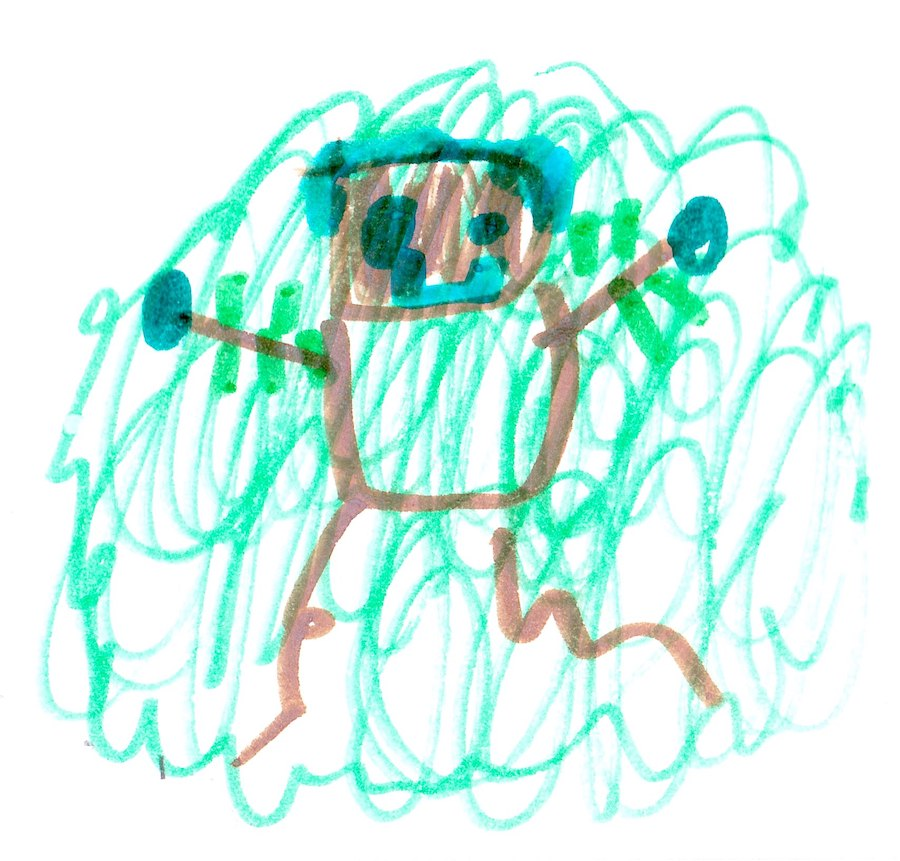
\includegraphics[width=4.16667in]{img/13-forcefield.jpg}
\caption{}
\end{figure}

\emph{One hour later\ldots{}}

I said, ``We are losing the battle.'' The Villagers saw and decided to
help. I said, ``The villagers were saved. Now it is just us and
Herobrine.''

\chapter{Herobrine and Us}\label{herobrine-and-us}

Our team thought we had the advantage but we were wrong. Soon everybody
was hurt but me. It was because of my life shield. I said, ``Guys we
can't give up.'' Then I saw the Fire Gem fly towards Felix. Then Felix
turned into the Fire God. Felix and I fought Herobrine but Felix wasn't
used to his power so after a while he would lose his power. As soon as
Felix lost his power Herobrine picked up the Fire Gem and said,
``Yes\ldots{}more\ldots{}MORE!'' as he turned into the Fire God.

\begin{figure}
\centering
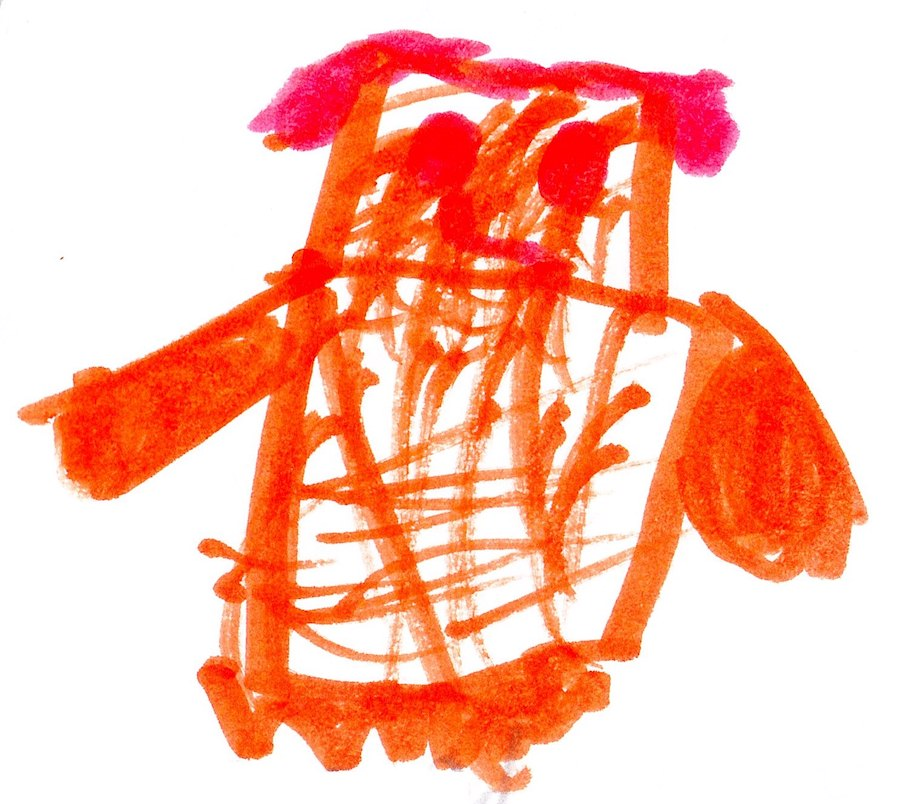
\includegraphics[width=3.12500in]{img/15-orangeguy.jpg}
\caption{}
\end{figure}

I called Everyone else and said, ``Help!'' Everyone came. Then a portal
opened. I said, ``Steve, I was wondering where the Magic Gem was, and
now I know you are the magic god.'' he hit Herobrine but it didn't do a
dent. Then Herobrine got his power too. The magic got turned back into
Steve. Herobrine destroyed Malek and hope was lost. The fight went on at
the end. Herobrine punched me so hard that I turned back into a human.
But Herobrine couldn't find the Life Gem, so he got the life lock key
from our base instead. Herobrine had won.

\chapter{The New World}\label{the-new-world}

Felix was in a secret base when the door opened. Malek said, ``Herobrine
destroyed the last town.'' Felix said, ``Herobrine got the life lock key
and killed Beckett; now he has the upper hand.''

\begin{figure}
\centering
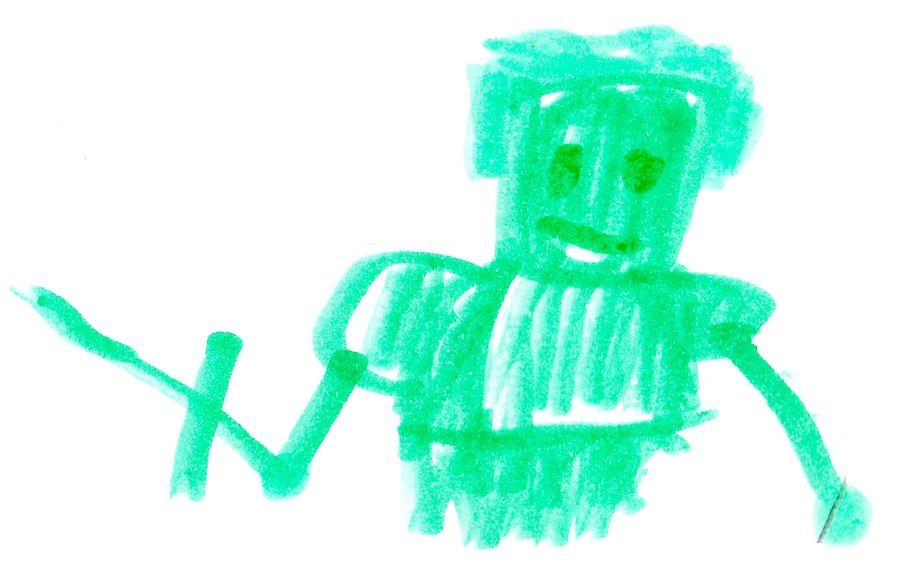
\includegraphics[width=4.16667in]{img/17-greenguy.jpg}
\caption{}
\end{figure}

\emph{At the bad guys base\ldots{}}

Herobrine said, ``It has been a year since I killed Beckett and I still
can't find the Life Gem.'' I hid it in my palm. Suddenly, I came back to
life as the Life God. I said, ``The Life Gem must have turned me alive
again.'' I went back to Felix's base and found Felix. We talked and
talked, and then I said, ``That's it! I'll talk to Cindy and Will and
see if they want to take down Herobrine.''

\chapter{Will or Will Not}\label{will-or-will-not}

\emph{In the Nether\ldots{}}

Will and Cindy were playing when I came. Will said, ``What do you
want?'' I said, ``Herobrine is destroying our land.'' Will said,
``Herobrine is destroying the Nether, too.'' I said, ``Then let's stop
Herobrine once and for all!''

Cindy and I will team up to the destroy Herobrine. Cindy took off her
mask. I said, ``Mom?'' Cindy said, ``Yes, Herobrine forced me to give up
all good and take on this disguise, or else I would die.'' Then Mom got
the Water Gem turned into the water God.

\chapter{The Last War}\label{the-last-war}

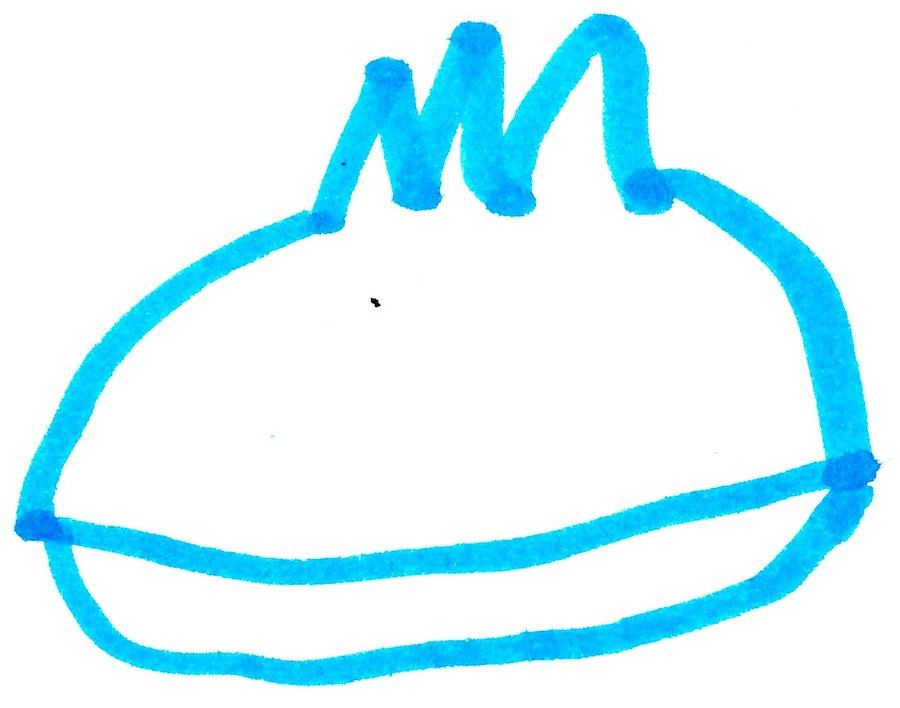
\includegraphics[width=0.78125in]{img/weapons-blueball.jpg}
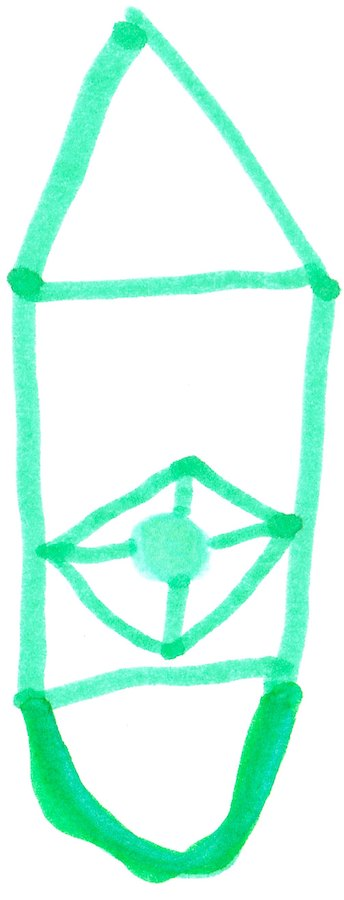
\includegraphics[width=0.31250in]{img/weapons-green.jpg}
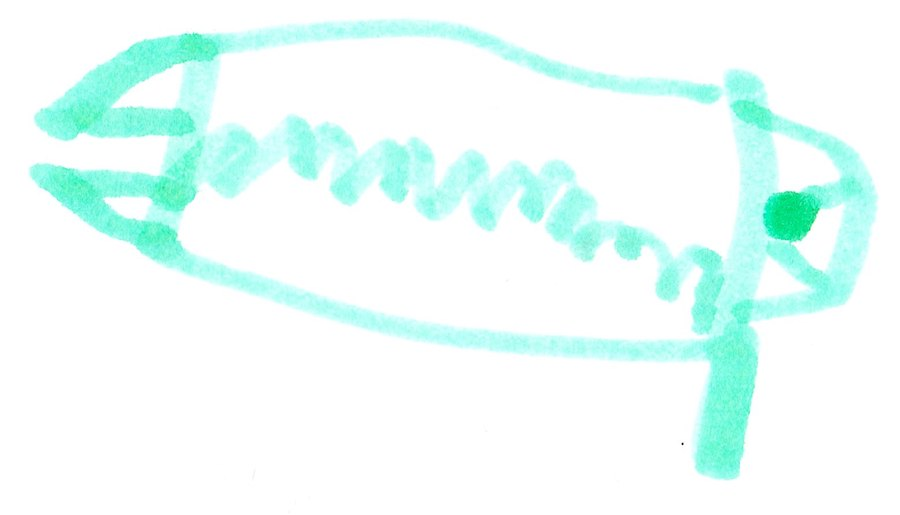
\includegraphics[width=0.78125in]{img/weapons-greengun.jpg}
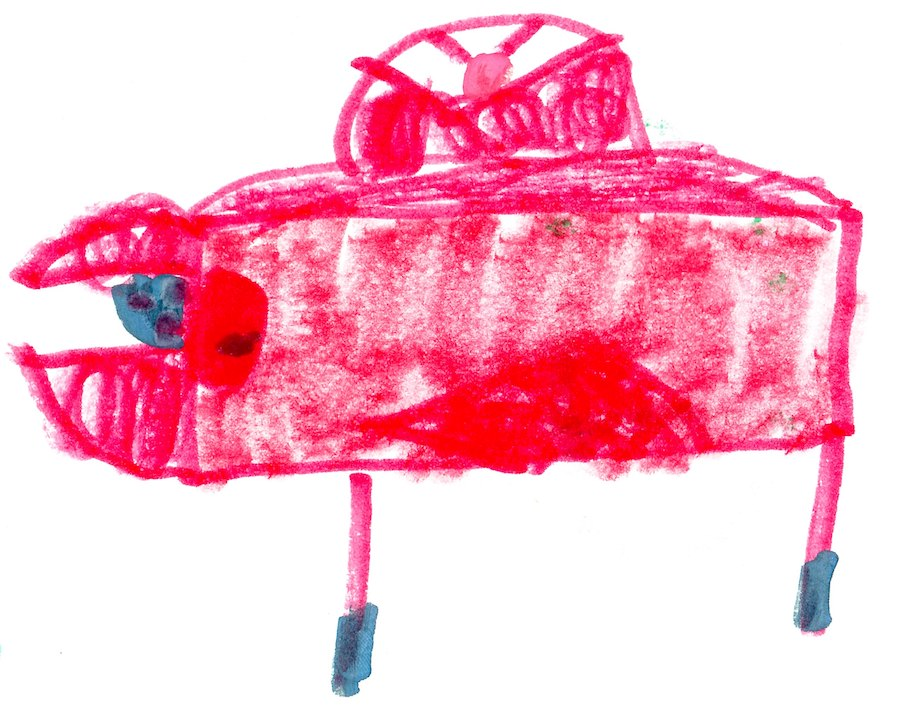
\includegraphics[width=0.78125in]{img/weapons-redguy.jpg}
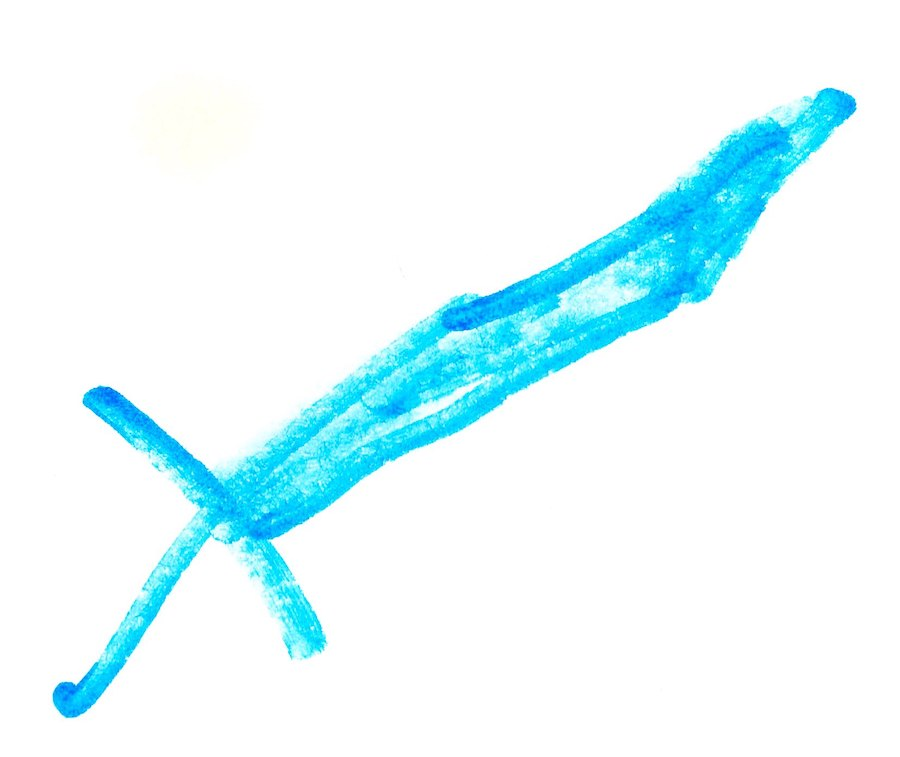
\includegraphics[width=0.78125in]{img/weapons-sword.jpg}

Malek turned into the night God. I got my life sword; Malek got his
night arrows and a night bow; and Mom got the ice machine. Suddenly
Herobrine came out of a portal. Will said, ``Herobrine, you boss us
around too much, now it's time for you to die.''

After a while Will destroyed his own heart -- the Nether Star -- to save
us all. Will's death caused Herobrine to lose the Fire Gem. Felix got
the Fire Gem and turned into the Fire God.

Eventually all of us were not able to fight. Dad as a ghost possessed me
and fought Herobrine. Felix said, ``Wow, I never knew dad was so
strong.'' But Herobrine still took Dad down. Then I had an idea.

I fought for a while and then shut my eyes. Felix said, ``Don't do it!''
Herobrine tried to punch me. I dodged it. Herobrine said, ``What? He had
his eyes closed.'' After a while I open my eyes and threw a magic ball
at Herobrine. Herobrine fell, and I cut his head to pieces. My team got
the life lock key and saved the world.

From that day on we were called\ldots{}

\textbf{WORLD'S DEFENDERS}

\end{document}
